\documentclass[utf8x, notes=hide]{beamer}

%\usepackage[bars]{beamerthemetree} % Beamer Theme v 2.2
\usetheme{boxes} % Beamer theme
\usecolortheme{seahorse} % Beamer color theme
% whale

\usepackage[boldfont,slantfont]{xeCJK}
\usepackage{fontspec}
\setmainfont{DejaVu Serif}
\setsansfont{DejaVu Sans}
\setmonofont{DejaVu Sans Mono}%{Monaco}
\setCJKmainfont{WenQuanYi Zen Hei}
\setCJKsansfont{WenQuanYi Macro Hei}
\setCJKmonofont{WenQuanYi Micro Hei Mono}
\setCJKfamilyfont{tt}{Monaco}

\usepackage{color}
\definecolor{listinggray}{gray}{0.9} 
\usepackage{xcolor}

\usepackage{listings}
% \lstset{numbers=left,
% backgroundcolor=\color{listinggray},
% frame=single,
% framexleftmargin=7mm,
% frameshape={RYN}{y}{y}{RYN}}
\usepackage{hyperref}
\usepackage{graphicx}

\title{Objective C 与 XCode}
\author[刘鑫]{刘鑫 <march@xiachufang.com>}
\institute{iOS 及 Mac OS 开发简介}

\begin{document}

\frame{\titlepage}

\begin{frame}
  \frametitle{关于本课程}
一个人应该能够换尿布,策划战争,杀猪,开船,设计房子,写十四行诗,结算
账户,砌墙,接脱臼的骨头,安慰濒死的人,服从命令,发布命令,携手合作,
独立行动,解数学方程,分析新问题,铲粪,电脑编程,做出可口的饭,善打架,
勇敢地死去。只有昆虫才专业化。\\
\rightline{——Robert A. Heinlein}
\end{frame}

%------------------------------------------
\section{Apple 硬件体系}
\begin{frame}
  \begin{center}
\begin{Huge}
What's Apple?
\end{Huge}
  \end{center}
\end{frame}
%------------------------------------------
\begin{frame}
\frametitle{肾之天敌}
  \begin{figure}
    \centering
    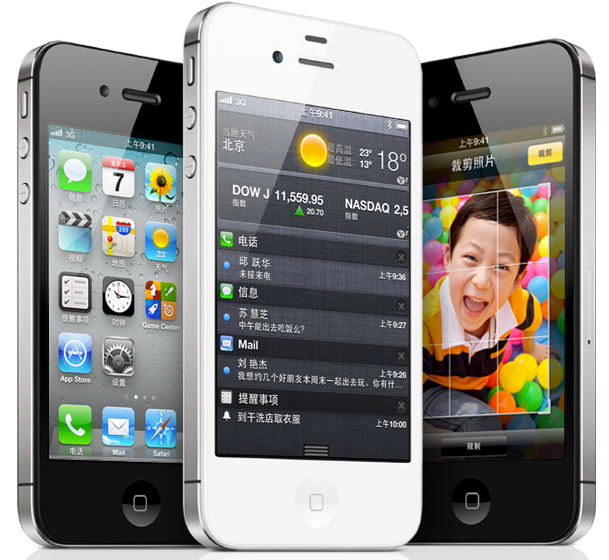
\includegraphics[bb=0 0 609 560,scale=.2]{images/iPhone.png}
    \caption{iPhone}
    \label{fig:iPhone}
  \end{figure}
\end{frame}
%------------------------------------------
\begin{frame}
\frametitle{一个卖 mp3 的公司居然咸鱼翻身了……——孔老师}
  \begin{figure}
    \centering
    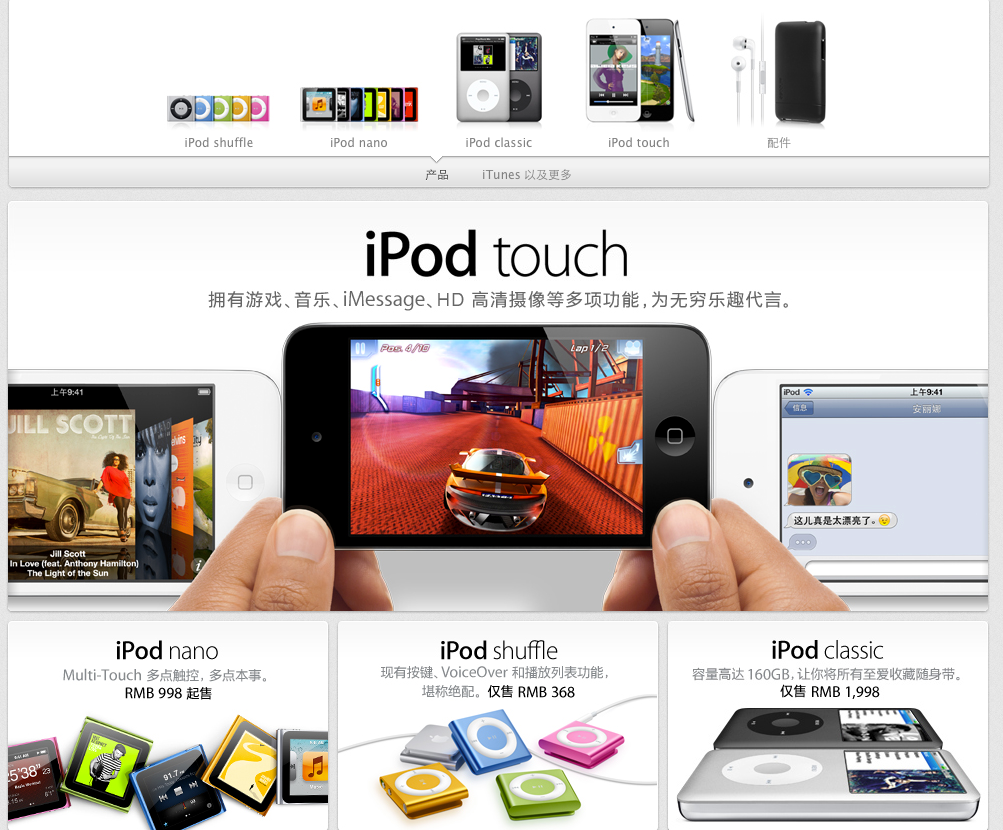
\includegraphics[bb=0 0 1003 830,scale=.2]{images/iPod.png}    
    \caption{iPod}
    \label{fig:iPod}
  \end{figure}
\end{frame}
%------------------------------------------
\begin{frame}
\frametitle{唯冠出品,中华之光}
  \begin{figure}
    \centering
    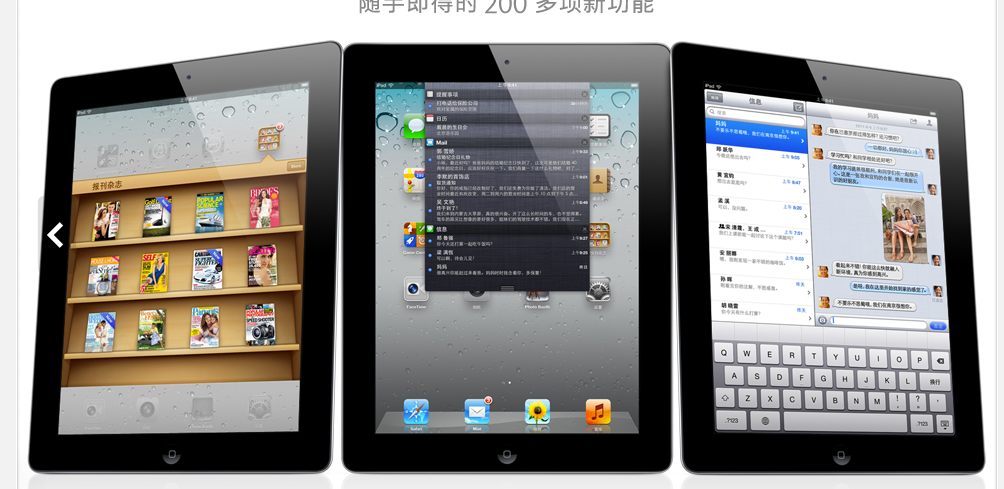
\includegraphics[bb=0 0 1004 489,scale=.2]{images/iPad.png}
    \label{fig:iPad}
  \end{figure}
\end{frame}
%------------------------------------------
\begin{frame}
  \frametitle{星巴克利器}
  \begin{figure}
    \centering
    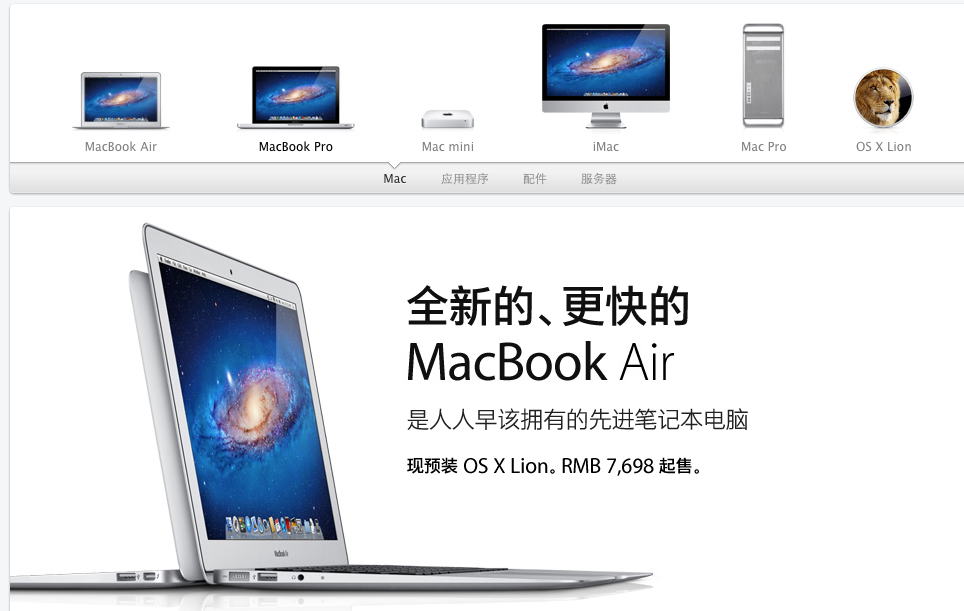
\includegraphics[bb=0 0 964 611,scale=.2]{images/mac.png}
    \label{fig:mac}
    \caption{各种 MAC}
    \label{fig:Mac}
  \end{figure}
\end{frame}
%------------------------------------------
\section{Apple 的软件体系}
\begin{frame}
\begin{center}
  \Huge{Apple 的软件体系}
\end{center}
\end{frame}
%------------------------------------------
\begin{frame}
  \frametitle{iOS —— mp3 厂商咸鱼翻身之秘}
  \begin{figure}
    \centering
    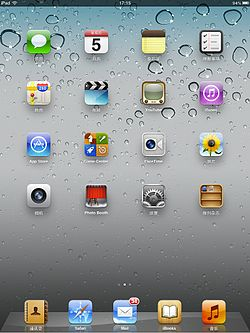
\includegraphics[bb=0 0 250 333,scale=.2]{images/iossoft.jpg}
    \caption{iOS 丰富的 APP}
    \label{fig:iossoft}
  \end{figure}
\end{frame}
%------------------------------------------
\begin{frame}
  \frametitle{Mac OS—— Alan Kay 抄袭了它}
  \begin{figure}
    \centering
    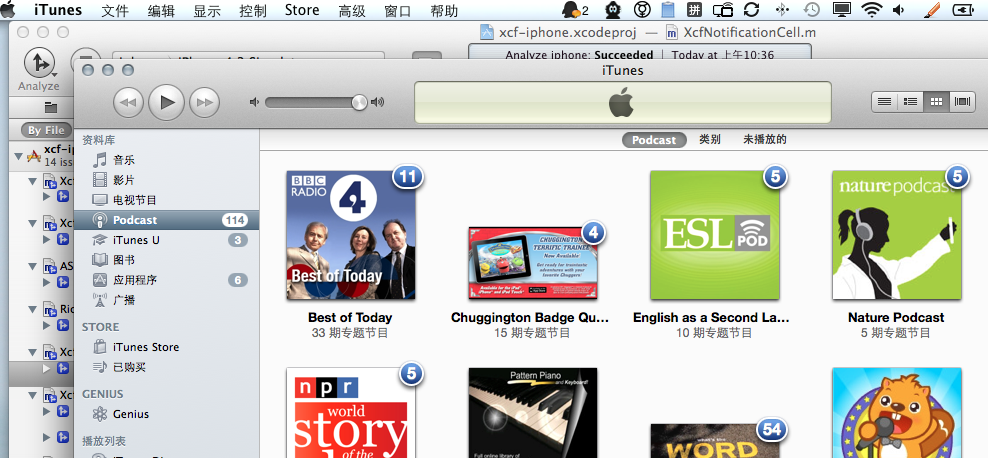
\includegraphics[bb=0 0 988 458,scale=.2]{images/macsoft.png}
    \caption{Mac OS 的软件正在向 iOS 风格转变}
    \label{fig:MacSoft}
  \end{figure}
\end{frame}
%------------------------------------------
\section{Apple 体系开发技术}
\begin{frame}[containsverbatim]
  \frametitle{Objective C}
  \begin{lstlisting}
#import <stdio.h>

int main(int argc, char* argv[]){
    printf("hello world!\n");
    return 0;
}
  \end{lstlisting}
\end{frame}
%------------------------------------------
\begin{frame}
  \frametitle{这货不是C}
  \begin{center}
  \begin{huge}
    等等,哪里不对?
  \end{huge}
  \end{center}
\end{frame}
%------------------------------------------
\begin{frame}
  \frametitle{这货真的不是C}
Objective C 是 C 语言的一个 Smalltalk 风格的面向对象扩展,高度兼容 C。
是 Apple 各平台的主力开发工具。
\end{frame}
%------------------------------------------
\begin{frame}[containsverbatim]
\frametitle{IDE 实作}
\begin{lstlisting}
#import <Foundation/Foundation.h>

int main (int argc, const char * argv[])
{

    @autoreleasepool {
        NSLog(@"Hello, World!");
        
    }
    return 0;
}
\end{lstlisting}
\end{frame}
%------------------------------------------
\begin{frame}
  \frametitle{XCode}
  XCode 是 Apple 官方推出的 Apple 体系开发工具,用于开发 Apple 各平台
  的 IDE。
\end{frame}

\section{操作演示阶段}
%------------------------------------------
\begin{frame}
  \frametitle{iOS 开发演示}
演示最简单的 ios 项目。
\end{frame}

%------------------------------------------
\begin{frame}
  \frametitle{来一发吧!}
演示最简单的 ios 项目建立。
\end{frame}

%------------------------------------------
\begin{frame}
  \frametitle{Objective?}
演示最简单的类型定义。
\end{frame}

%------------------------------------------
\begin{frame}
  \frametitle{GUI?}
演示最简单的 cocoa 界面开发。
\end{frame}

%------------------------------------------
\begin{frame}
  \frametitle{MVC?}
演示并解说 cocoa 的 MVC 结构。
\end{frame}

%------------------------------------------
\begin{frame}
  \frametitle{事件?}
演示并解说 cocoa 的事件绑定。
\end{frame}

%------------------------------------------
\begin{frame}
  \frametitle{Debug?}
演示并解说 cocoa 的一些 debug 操作。
\end{frame}

%------------------------------------------
\begin{frame}
  \frametitle{谁动了我的内存?}
Objective C 的内存管理基于 alloc/dealloc 机制。需要程序员细心管理。
\end{frame}

%------------------------------------------
\begin{frame}
  \frametitle{谁动了我的对象?}
Objective C 通过 init/release 机制管理对象结构的构造和释放。
\end{frame}

%------------------------------------------
\begin{frame}
  \frametitle{谁动了我的引用技术?}
Objective C 通过 retain/release 机制管理对象结构的构造和释放。
\end{frame}

%------------------------------------------
\begin{frame}
  \frametitle{谁动了我的属性?}
  \begin{itemize}
  \item retain/assign
  \item strong/weak
  \end{itemize}
\end{frame}

%------------------------------------------
\begin{frame}
  \frametitle{autorelease?}
AutoRelease 机制适用长生命周期的对象,不建议过度使用。
\end{frame}

%------------------------------------------
\begin{frame}
  \frametitle{托管给工具?}
GC 机制性能底下,新项目建议使用 arc 机制。
\end{frame}

%------------------------------------------
\begin{frame}
  \frametitle{我的内存哪儿去了?}
介绍 profile 工具
\end{frame}

%------------------------------------------
\begin{frame}
  \frametitle{我的代码可靠吗?}
介绍 analyze 工具。
\end{frame}

%------------------------------------------
\begin{frame}
  \frametitle{我的项目质量高吗?}
介绍 Unit Test 工具 GHUnitTest。
\end{frame}


\section{学习 Apple 开发体系}
%------------------------------------------
\begin{frame}
  \begin{center}
推荐开发书籍。
  \end{center}
\end{frame}

\begin{frame}
  \begin{center}
我们的项目中使用的第三方组件。
  \end{center}
\end{frame}

\begin{frame}
  \frametitle{再见!}
  \begin{center}
    谢谢大家!\\
\rightline{Power By \LaTeX{}}
  \end{center}
\end{frame}

\end{document}